\documentclass[11pt]{article}
\usepackage{color, array, graphics}
\usepackage{enumerate}
\usepackage{mathtools}
\usepackage{fullpage}
\usepackage[utf8]{inputenc}
\usepackage{amsmath}
\usepackage{tikz}

%Symbol shortcuts
\def\OR{\vee}
\def\AND{\wedge}
\def\imp{\rightarrow}

%Aesthetics
\addtolength{\oddsidemargin}{-.5in}
\addtolength{\evensidemargin}{-.5in}

\addtolength{\topmargin}{-.5in}


\begin{document}

\textbf{Alexander Garcia}

21 April 2017 \\

	\begin{enumerate}

		\item Question 1

			\begin{enumerate}[(a)]

				\item When rolling the Zocchihedron the first time, you are guaranteed to get a number.
					The probability of rolling the same number in any of the next four rolls is
					$\frac{1}{100}$. The sum of these probabilities is $\frac{4}{100} = \frac{1}{25} = 0.04$\\

				\item A fair die will have exactly $\frac{1}{100}$ chance of rolling a given number.
					Using the same logic as in part (a), we must solve for the number of rolls, rather
					than the probability.

					$\frac{n}{100} = 0.3$

					$n = 30$ rolls \\


			\end{enumerate}

\newpage

\textbf{Alexander Garcia}

21 April 2017 \\

		\item Question 2

			\begin{enumerate}[(a)]

				\item Probability Distribution: $\sum_{s \in S}{p(s)} = 1$

					$p(100) = 5p(n), n \in \{1, 2, \cdots, 99\}$

					$p(1) = p(2) = \cdots = p(99)$

					$99*p(1) + 5*p(1) = 1$

					$104*p(1) = 1$ \\

					$p(i) = \frac{1}{104}, i \in \{1, 2, \cdots, 99\}$

					$p(100) = \frac{5}{104}$ \\

				\item For any one roll, the $p(100) = \frac{5}{104}$. Thus, the
					probability of rolling a 100 in any n rolls is $\frac{5n}{104}$, since
					the probability each time compounds, adding another $\frac{5}{104}$

			\end{enumerate}
\newpage
\textbf{Alexander Garcia}

21 April 2017 \\

		\item Question 3

			\begin{enumerate}[(a)]

				\item In order for a bit string of length $n$ to contain an equal number of 1's and 0's,
					it must have $\frac{n}{2}$ of each (1, 0 are treated as heads and tails over n flips).
					For a bit string of length $n$ there are $C(n, \frac{n}{2})$ strings with equal 1's and
					0's.

					There are $2^n$ total possible outcomes of flipping the coin $n$ times, and
					$C(n, \frac{n}{2})$ of these will have an even number of heads and tails.

					The probability is then $\frac{\frac{n!}{(n/2)!(n/2)!}}{2^n} $. \\

				\item It will not affect the original probability.

					Limiting the first flip to heads limits the number of total
					possible outcomes to $2^{n-1}$.

					Of the remaining flips, there must be exactly one more tail result than heads.
					This number of strings is $C(n-1, \lceil{\frac{n}{2} -1}\rceil)$, where
					$\lceil{\frac{n}{2} -1}\rceil = \frac{n-1}{2}$, since $n$ must be odd.

					Probability = $\frac{\frac{(n-1)!}{(\frac{n-1}{2})!(\frac{n-1}{2})!}}{2^{n-1}}
					* \frac{\frac{n}{n/2}}{2} = \frac{\frac{n!}{(n/2)!(n/2)!}}{2^n} $

					Since the ratios are the same, the probabilities are the same. \\

				\item $E(X) = \sum_{t \in S}{p(t)X(t)}$

					$X(t) = \sum_{i = 1}^{n}X_i(t)$

					$E(X) = \sum_{i = 1}^{n}{(\sum_{j = 1}^{i}{0.5 * 2} + \sum_{j = 1}^{i}{0.5 * -1})}$

					$=\sum_{i = 1}^{n}{i - \frac{i}{2} } = \sum_{i = 1}^{n}{\frac{i}{2} }$ \\

					The expected value is the sum of all the possibilities that the random variable $X(T)$ can take,
					weighted by their probabilities. There is a $0.5$ probability that a flip will come up heads, and the
					same for tails. Here, $n$ would be the maximum number of flips, and $i$ is the number of flips for
					the current trial.

			\end{enumerate}
\newpage
\textbf{Alexander Garcia}

21 April 2017 \\

		\item Question 4

			Use Bayes' Theorem

			$E:=$ the storm produces hail

			$F:=$ the storm is a supercell storm

			\begin{tabular}{ll}

				$P(F) = \frac{1}{1000} = 0.001$ & Probability of there being a supercell storm \\

				$P(E|F) = 0.75$ & Probability of it hailing during a supercell storm \\

				$P(\neg F) = 1-0.001 = 0.999$ & Probability of there not being a supercell storm \\

				$P(E|\neg F) = 0.15$ & Probability of it not hailing during a supercell storm \\

			\end{tabular}

			$P(F|E) = \frac{P(E|F)*P(F)}{P(E|F)*P(F) + P(E|\neg F)*P(\neg F)}$

			$=\frac{0.75 * 0.001}{0.75 * 0.001 + 0.15 * 0.999} = 0.00498 = 0.5\%$ chance that the hail is from
			a supercell storm.

\newpage
\textbf{Alexander Garcia}

21 April 2017 \\

		\item Question 5


			\begin{center}
			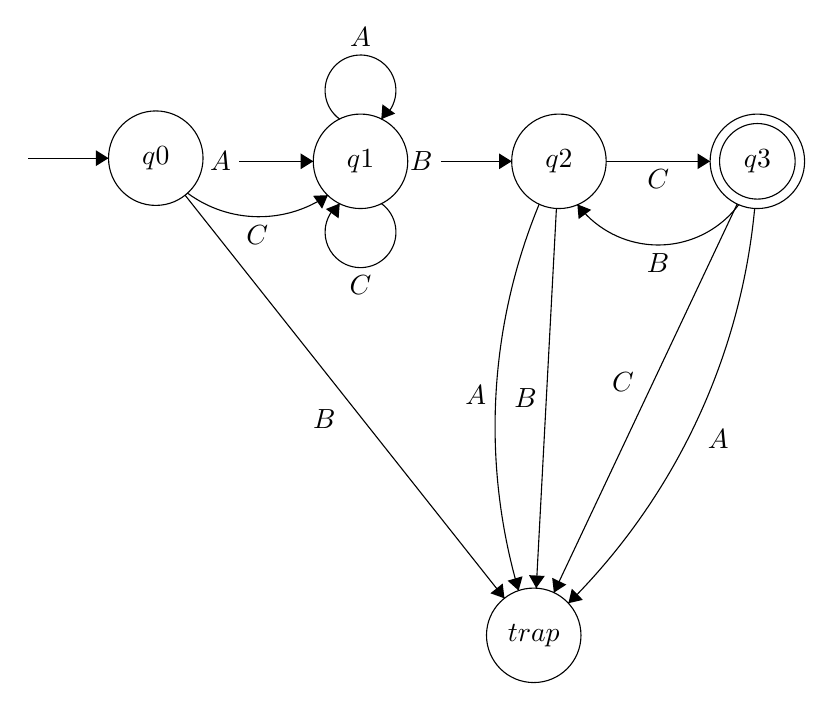
\begin{tikzpicture}[scale=0.2]
				\tikzstyle{every node}+=[inner sep=0pt]
				\draw [black] (14.3,-11.1) circle (3);
				\draw (14.3,-11.1) node {$q0$};
				\draw [black] (27.3,-11.3) circle (3);
				\draw (27.3,-11.3) node {$q1$};
				\draw [black] (39.9,-11.3) circle (3);
				\draw (39.9,-11.3) node {$q2$};
				\draw [black] (52.5,-11.3) circle (3);
				\draw (52.5,-11.3) node {$q3$};
				\draw [black] (52.5,-11.3) circle (2.4);
				\draw [black] (38.3,-41.4) circle (3);
				\draw (38.3,-41.4) node {$trap$};
				\draw [black] (6.2,-11.1) -- (11.3,-11.1);
				\fill [black] (11.3,-11.1) -- (10.5,-10.6) -- (10.5,-11.6);
				\draw [black] (19.6,-11.3) -- (24.3,-11.3);
				\draw (19.1,-11.3) node [left] {$A$};
				\fill [black] (24.3,-11.3) -- (23.5,-10.8) -- (23.5,-11.8);
				\draw [black] (25.233,-13.447) arc (-55.15159:-126.61122:7.649);
				\fill [black] (25.23,-13.45) -- (24.29,-13.49) -- (24.86,-14.31);
				\draw (20.74,-15.34) node [below] {$C$};
				\draw [black] (25.977,-8.62) arc (234:-54:2.25);
				\draw (27.3,-4.05) node [above] {$A$};
				\fill [black] (28.62,-8.62) -- (29.5,-8.27) -- (28.69,-7.68);
				\draw [black] (28.623,-13.98) arc (54:-234:2.25);
				\draw (27.3,-18.55) node [below] {$C$};
				\fill [black] (25.98,-13.98) -- (25.1,-14.33) -- (25.91,-14.92);
				\draw [black] (32.4,-11.3) -- (36.9,-11.3);
				\draw (31.9,-11.3) node [left] {$B$};
				\fill [black] (36.9,-11.3) -- (36.1,-10.8) -- (36.1,-11.8);
				\draw [black] (16.16,-13.45) -- (36.44,-39.05);
				\fill [black] (36.44,-39.05) -- (36.33,-38.11) -- (35.55,-38.73);
				\draw (25.74,-27.67) node [left] {$B$};
				\draw [black] (51.331,-14.033) arc (-36.61287:-143.38713:6.392);
				\fill [black] (41.07,-14.03) -- (41.15,-14.97) -- (41.95,-14.38);
				\draw (46.2,-17.11) node [below] {$B$};
				\draw [black] (42.9,-11.3) -- (49.5,-11.3);
				\fill [black] (49.5,-11.3) -- (48.7,-10.8) -- (48.7,-11.8);
				\draw (46.2,-11.8) node [below] {$C$};
				\draw [black] (37.34,-38.559) arc (-163.65353:-202.43199:37.004);
				\fill [black] (37.34,-38.56) -- (37.59,-37.65) -- (36.64,-37.93);
				\draw (35.32,-26.15) node [left] {$A$};
				\draw [black] (39.74,-14.3) -- (38.46,-38.4);
				\fill [black] (38.46,-38.4) -- (39,-37.63) -- (38,-37.58);
				\draw (38.52,-26.32) node [left] {$B$};
				\draw [black] (52.329,-14.294) arc (-5.37996:-45.13224:40.765);
				\fill [black] (40.5,-39.36) -- (41.42,-39.15) -- (40.72,-38.44);
				\draw (49.32,-28.92) node [right] {$A$};
				\draw [black] (51.22,-14.01) -- (39.58,-38.69);
				\fill [black] (39.58,-38.69) -- (40.37,-38.18) -- (39.47,-37.75);
				\draw (44.69,-25.3) node [left] {$C$};
			\end{tikzpicture}

		\end{center}
		\newpage
\textbf{Alexander Garcia}

21 April 2017 \\

		\item Question 6

			\begin{enumerate}[(a)]

				\item $L(M) = (0^*10^*10^*)^*00$

				\item NFA\\

					\begin{center}
						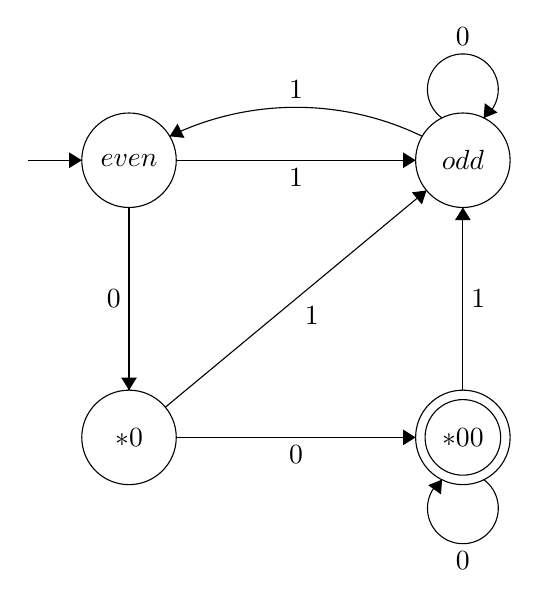
\begin{tikzpicture}[scale=0.2]
							\tikzstyle{every node}+=[inner sep=0pt]
							\draw [black] (11,-10.9) circle (3);
							\draw (11,-10.9) node {$even$};
							\draw [black] (32.2,-10.9) circle (3);
							\draw (32.2,-10.9) node {$odd$};
							\draw [black] (11,-28.5) circle (3);
							\draw (11,-28.5) node {$*0$};
							\draw [black] (32.2,-28.5) circle (3);
							\draw (32.2,-28.5) node {$*00$};
							\draw [black] (32.2,-28.5) circle (2.4);
							\draw [black] (14,-10.9) -- (29.2,-10.9);
							\fill [black] (29.2,-10.9) -- (28.4,-10.4) -- (28.4,-11.4);
							\draw (21.6,-11.4) node [below] {$1$};
							\draw [black] (11,-13.9) -- (11,-25.5);
							\fill [black] (11,-25.5) -- (11.5,-24.7) -- (10.5,-24.7);
							\draw (10.5,-19.7) node [left] {$0$};
							\draw [black] (14,-28.5) -- (29.2,-28.5);
							\fill [black] (29.2,-28.5) -- (28.4,-28) -- (28.4,-29);
							\draw (21.6,-29) node [below] {$0$};
							\draw [black] (4.6,-10.9) -- (8,-10.9);
							\fill [black] (8,-10.9) -- (7.2,-10.4) -- (7.2,-11.4);
							\draw [black] (13.582,-9.378) arc (115.84321:64.15679:18.395);
							\fill [black] (13.58,-9.38) -- (14.52,-9.48) -- (14.08,-8.58);
							\draw (21.6,-7.04) node [above] {$1$};
							\draw [black] (30.877,-8.22) arc (234:-54:2.25);
							\draw (32.2,-3.65) node [above] {$0$};
							\fill [black] (33.52,-8.22) -- (34.4,-7.87) -- (33.59,-7.28);
							\draw [black] (13.31,-26.58) -- (29.89,-12.82);
							\fill [black] (29.89,-12.82) -- (28.96,-12.94) -- (29.6,-13.71);
							\draw (22.61,-20.19) node [below] {$1$};
							\draw [black] (32.2,-25.5) -- (32.2,-13.9);
							\fill [black] (32.2,-13.9) -- (31.7,-14.7) -- (32.7,-14.7);
							\draw (32.7,-19.7) node [right] {$1$};
							\draw [black] (33.523,-31.18) arc (54:-234:2.25);
							\draw (32.2,-35.75) node [below] {$0$};
							\fill [black] (30.88,-31.18) -- (30,-31.53) -- (30.81,-32.12);
						\end{tikzpicture}
					\end{center}

			\end{enumerate}

	\end{enumerate}

\end{document}


